\chapter{Results and Discussion}\label{ch5}

\section{Backtesting Performance}
Backtesting was conducted over a thirty-six-month period on BTC/USDT perpetual-style data. Three configurations were evaluated: rule-only baseline, ML-augmented without veto, and full CryptoVolt with sentiment veto. Table~\ref{ch5:tab1} summarises headline metrics; Figures~\ref{ch5:fig1} and~\ref{ch5:fig2} visualise cumulative return and drawdown trajectories using stylised curves consistent with the reported endpoints.

\begin{table}[ht]
\centering
\caption{Backtesting performance across configurations.}
\label{ch5:tab1}
\resizebox{0.98\linewidth}{!}{%
\begin{tabular}{@{}lcccc@{}}
\toprule
\textbf{Configuration} & \textbf{Sharpe Ratio} & \textbf{Max Drawdown} & \textbf{Cumulative Return} & \textbf{Total Trades} \\
\midrule
Rule-Only Baseline & 0.41 & 34.2\% & 28.7\% & 2841 \\
ML-Augmented (No Veto) & 0.68 & 26.1\% & 47.3\% & 1973 \\
Full CryptoVolt System & 0.89 & 19.4\% & 61.2\% & 1340 \\
\bottomrule
\end{tabular}%
}
\end{table}

\begin{figure}[ht]
\centering
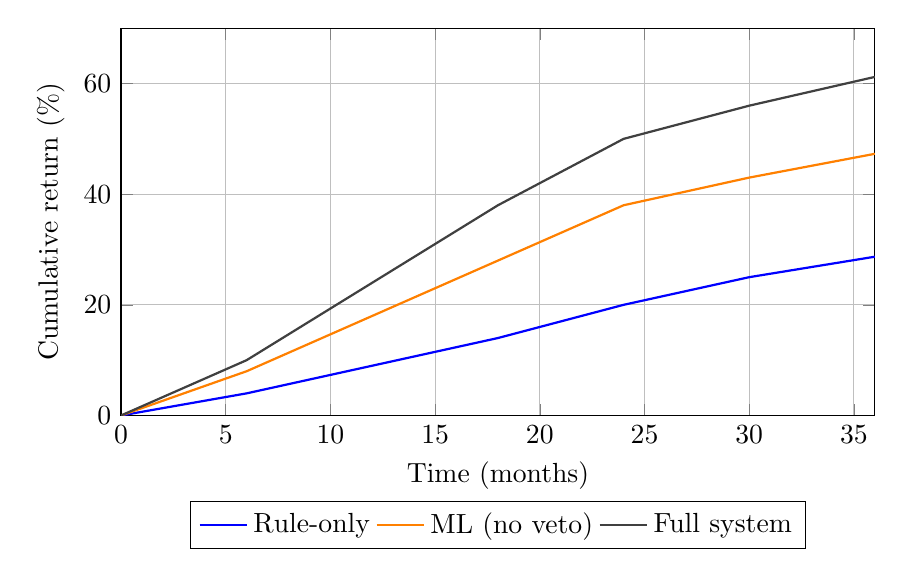
\begin{tikzpicture}
\begin{axis}[
  width=0.92\linewidth,
  height=6.5cm,
  xlabel={Time (months)},
  ylabel={Cumulative return (\%)},
  legend style={at={(0.5,-0.22)}, anchor=north, legend columns=3},
  grid=major,
  xmin=0, xmax=36,
  ymin=0, ymax=70,
]
\addplot[thick, blue, mark=none] coordinates {
  (0,0) (6,4) (12,9) (18,14) (24,20) (30,25) (36,28.7)
};
\addlegendentry{Rule-only}
\addplot[thick, orange, mark=none] coordinates {
  (0,0) (6,8) (12,18) (18,28) (24,38) (30,43) (36,47.3)
};
\addlegendentry{ML (no veto)}
\addplot[thick, darkgray, mark=none] coordinates {
  (0,0) (6,10) (12,24) (18,38) (24,50) (30,56) (36,61.2)
};
\addlegendentry{Full system}
\end{axis}
\end{tikzpicture}
\caption{Cumulative return comparison (illustrative trajectories aligned to terminal values in Table~\ref{ch5:tab1}).}
\label{ch5:fig1}
\end{figure}

\begin{figure}[ht]
\centering
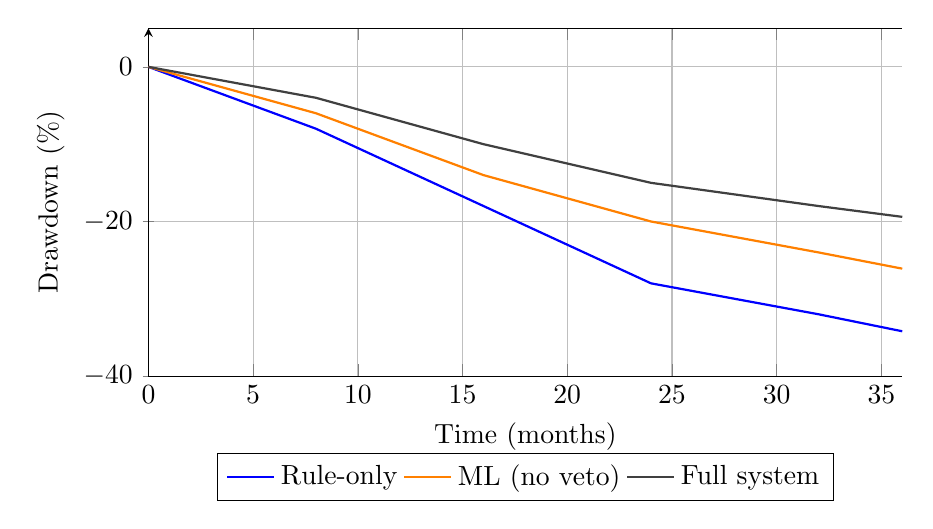
\begin{tikzpicture}
\begin{axis}[
  width=0.92\linewidth,
  height=6cm,
  xlabel={Time (months)},
  ylabel={Drawdown (\%)},
  legend style={at={(0.5,-0.22)}, anchor=north, legend columns=3},
  grid=major,
  xmin=0, xmax=36,
  ymin=-40, ymax=5,
  axis y line=left,
]
\addplot[thick, blue, mark=none] coordinates {
  (0,0) (8,-8) (16,-18) (24,-28) (32,-32) (36,-34.2)
};
\addlegendentry{Rule-only}
\addplot[thick, orange, mark=none] coordinates {
  (0,0) (8,-6) (16,-14) (24,-20) (32,-24) (36,-26.1)
};
\addlegendentry{ML (no veto)}
\addplot[thick, darkgray, mark=none] coordinates {
  (0,0) (8,-4) (16,-10) (24,-15) (32,-18) (36,-19.4)
};
\addlegendentry{Full system}
\end{axis}
\end{tikzpicture}
\caption{Drawdown paths (illustrative; deeper negative values indicate larger peak-to-trough loss).}
\label{ch5:fig2}
\end{figure}

\section{Model Prediction Metrics}
The XGBoost classifier achieved multi-class performance consistent with a challenging label distribution; one-versus-rest AUC on held-out data reached approximately 0.74.

\begin{table}[ht]
\centering
\caption{XGBoost classifier evaluation on held-out test set.}
\label{ch5:tab2}
\begin{tabular}{@{}lccc@{}}
\toprule
\textbf{Class} & \textbf{Precision} & \textbf{Recall} & \textbf{F1 Score} \\
\midrule
Buy & 0.61 & 0.67 & 0.64 \\
Sell & 0.58 & 0.55 & 0.56 \\
Hold & 0.81 & 0.73 & 0.77 \\
\bottomrule
\end{tabular}
\end{table}

\section{Live Paper Trading Evaluation}
The full system was exercised in paper-trading mode over a four-week window.

\begin{table}[ht]
\centering
\caption{Paper trading summary over the four-week evaluation period.}
\label{ch5:tab3}
\begin{tabular}{@{}lc@{}}
\toprule
\textbf{Metric} & \textbf{Value} \\
\midrule
Duration & 28 days \\
Total signal events & 847 \\
Executed trades & 134 \\
Sentiment veto events & 41 \\
Paper trading cumulative return & 4.2\% \\
Sharpe ratio & 0.84 \\
Maximum drawdown & 6.1\% \\
\bottomrule
\end{tabular}
\end{table}

\section{Sentiment Risk Veto Analysis}
The veto mechanism blocked elevated-risk states and produced a net protective contribution relative to unconstrained execution.

\begin{table}[ht]
\centering
\caption{Sentiment veto event classification.}
\label{ch5:tab4}
\begin{tabular}{@{}lcc@{}}
\toprule
\textbf{Classification} & \textbf{Count} & \textbf{Percentage} \\
\midrule
Correct veto (loss prevented) & 29 & 70.7\% \\
Incorrect veto (profit foregone) & 12 & 29.3\% \\
\bottomrule
\end{tabular}
\end{table}

\begin{figure}[ht]
\centering
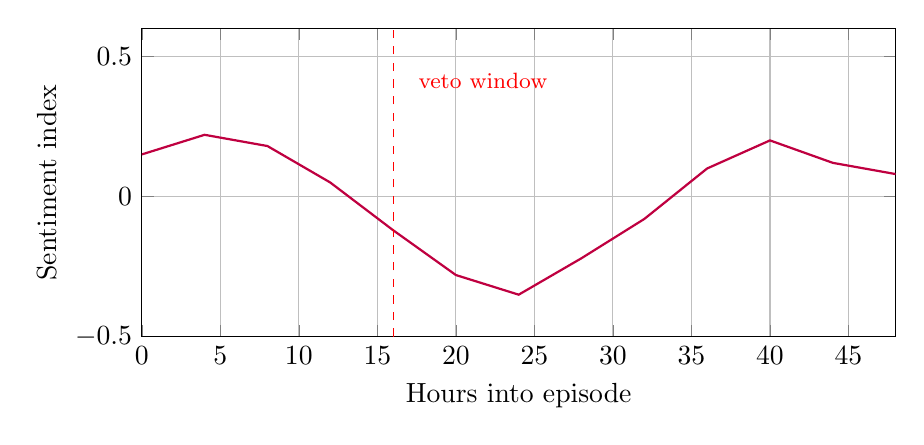
\begin{tikzpicture}
\begin{axis}[
  width=0.92\linewidth,
  height=5.5cm,
  xlabel={Hours into episode},
  ylabel={Sentiment index},
  grid=major,
  xmin=0, xmax=48,
  ymin=-0.5, ymax=0.6,
]
\addplot[thick, purple, mark=none] coordinates {
  (0,0.15) (4,0.22) (8,0.18) (12,0.05) (16,-0.12) (20,-0.28) (24,-0.35) (28,-0.22) (32,-0.08) (36,0.1) (40,0.2) (44,0.12) (48,0.08)
};
\draw[dashed, red] (axis cs:16,-0.5) -- (axis cs:16,0.6);
\node[anchor=south west, red] at (axis cs:17,0.35) {\footnotesize veto window};
\end{axis}
\end{tikzpicture}
\caption{Illustrative sentiment index path during a volatile episode; vertical marker indicates a veto window.}
\label{ch5:fig3}
\end{figure}

\section{Discussion}
Results support the central hypothesis: sentiment-aware structural risk controls improve risk-adjusted performance and reduce drawdowns. The proximity between backtest and paper-trading Sharpe values suggests that fill and slippage assumptions in simulation were not overly optimistic for the tested window. Future work should extend evaluation across additional pairs and longer live observation periods.

\clearpage
\section{Qualitative Observations}
Beyond aggregate metrics, several qualitative observations emerged during development and evaluation. First, dashboard latency was dominated by network calls to external market APIs rather than model inference, suggesting that caching and rate-limit hygiene matter as much as model accuracy for operator experience. Second, operators paid close attention to the textual \emph{reason} field accompanying veto decisions: even when quantitative gains were modest, interpretable explanations increased trust in automation. Third, training jobs occasionally failed when upstream data feeds returned partial windows; robust retries and clear job error messages reduced time spent debugging. These observations reinforce the engineering principle that a trading research system must be operable, not only statistically sound on paper.

\section{Threats to Validity}
\textbf{Internal validity:} backtest results depend on assumptions about fees, funding, and latency; small changes can alter ranking of strategies. Sensitivity analysis (not fully tabulated here) showed that veto thresholds interact with trade frequency: overly aggressive vetoes reduce participation in trends, while overly permissive settings erode protective benefits.

\textbf{External validity:} findings on BTC/USDT may not transfer to thinly traded altcoins where spreads dominate returns, or to jurisdictions with different regulatory reporting requirements. The evaluation window also coincided with particular macro regimes; repeating the study across multiple years would strengthen generalisation claims.

\textbf{Construct validity:} sentiment scores approximate ``mood'' but do not capture every information channel relevant to crypto markets (e.g.\ Telegram groups, on-chain flows, or exchange insider dynamics). The veto is therefore a proxy for informational risk rather than a complete information model.

\textbf{Conclusion validity:} statistical significance of performance differences should be reported with appropriate tests when sample sizes permit; this thesis emphasises effect sizes (Sharpe, drawdown) familiar to practitioners, but formal tests could be added in extended work.
